\chapter{Design}\label{design_ch}
\textbf{Til Jakob: Jeg overvejer om det her kapitel skal slåes sammen med impelementation da det er ret kort. I projectet har der jo mere været fokus på funktionaliteten frem for designet. Hvad tænker du? Hvordan kan man få mere kød på det her?}
TODO: Introduction to this Chapter, what to expect in this Chapter..


\section{Overview}
The solution that has been proposed is to use the gestures defined in Figure \ref{pitch} and \ref{roll} and instead of using a VAS. The orientation for each gesture should be translated to a value on a scale from zero to ten. To achieve this a wristband equipped with an IMU and a button will be used, the user will use one of the gestures and the press of the button to input the desired value. In order to view the data the wristband will a accompanied by a smartphone app, the companion app will display the logged data and offer the possibility to export it to a data file. This design is illustrated in Figure \ref{design_overview}.

Since the main focus of this report is to compare the gesture based input method to a VAS, the approach to the design of the companion app will be to create a Minimum Viable Product (MVP)\cite{mvp}. This means that it will focus a minimal set of features, just enough to be use able, like vise the user interface (UI) will be kept simple.

MVP!

\begin{figure}[h]
    \centering
    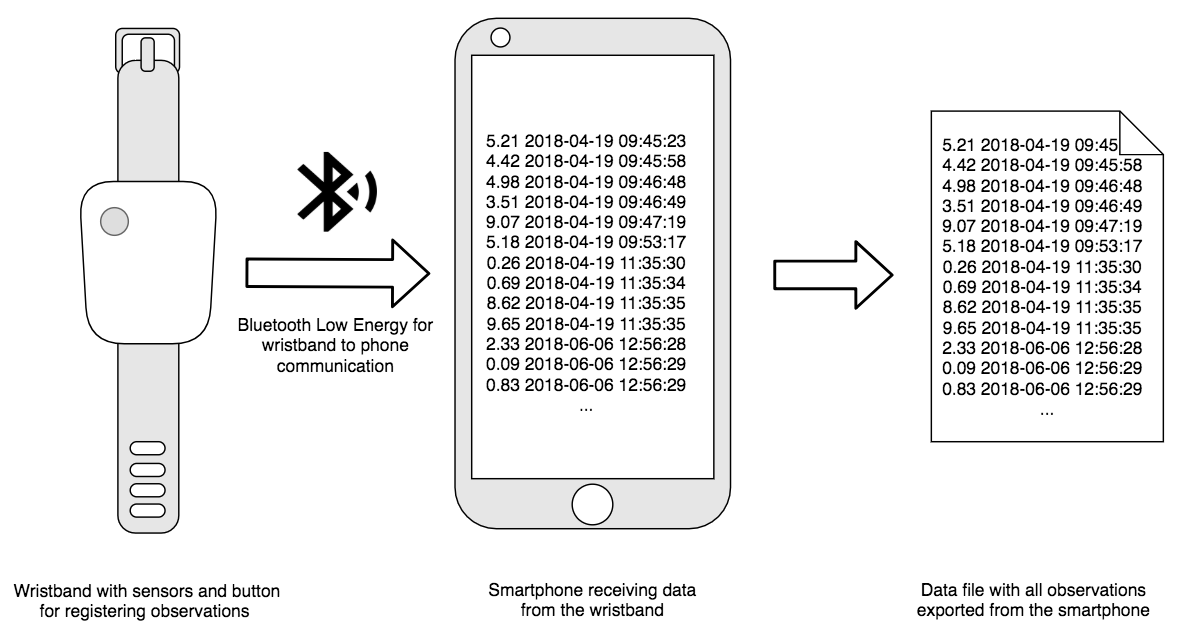
\includegraphics[width=1\textwidth]{figures/design_overview.png}
    \caption{Wristband device with sensors and a button for registering observation. Smartphone to import, display and export the data}
    \label{design_overview}
\end{figure}


\section{Functionalities \& Requirements}\label{requirements}
With the general outline for the wristband and companion app laid out, we can create a list of functionalities and requirements that shall be implemented in order to create a MVP.

\begin{itemize}
    \item \textbf{Log data:} The user should be able to log observation using the wristband, this should be possible to do independently from the companion app
    \item \textbf{Import data:} The companion app shall import the logged data from the wristband
    \item \textbf{Display data:} The companion app shall display the logged data (scaled value and time stamp)
    \item \textbf{Export data:} The companion app shall be able to export the logged data to a data file for further investigation
	\item \textbf{Simple solution:} It should be simple and easy to perform all of the above actions.
\end{itemize}